\subsection{CIAO Plots}

\begin{figure}[H]
    \begin{subfigure}{.4\textwidth}
        \centering
        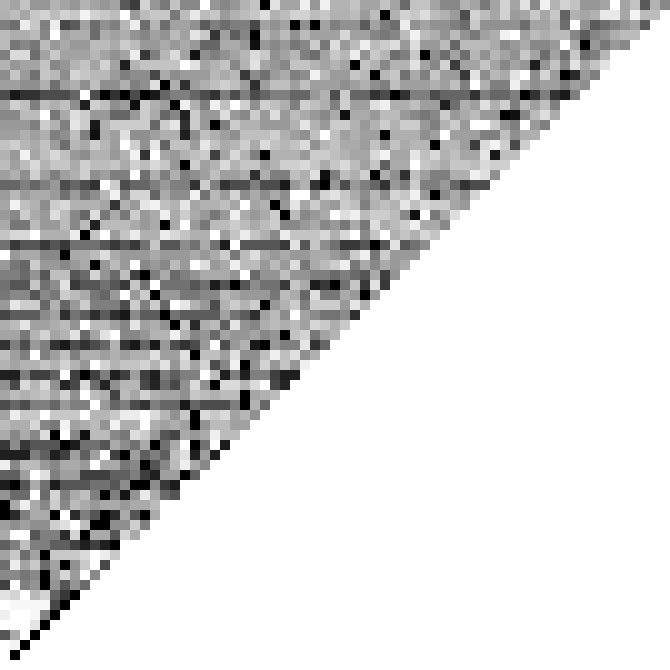
\includegraphics[width=.4\linewidth]{images/cycling/high_config_14.png}
        \caption{Generation 14 for High Configuration}
        \label{fig:sfig1}
    \end{subfigure}
    \begin{subfigure}{.4\textwidth}
        \centering
        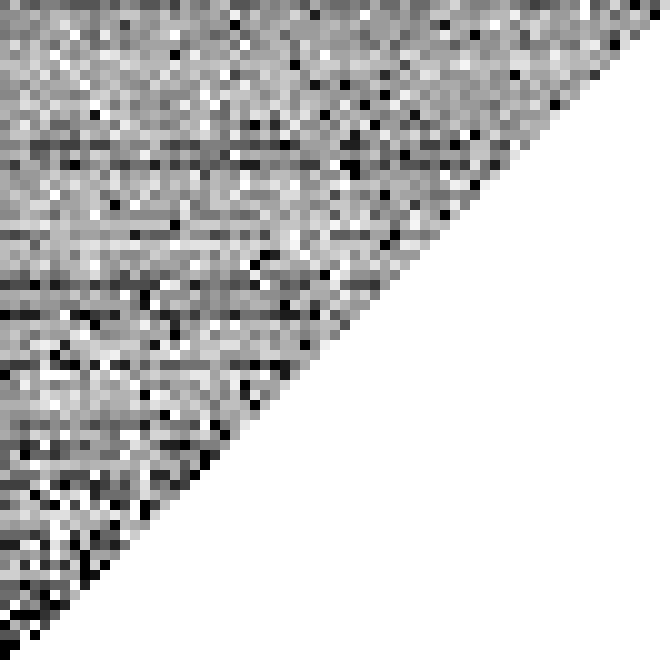
\includegraphics[width=0.4\linewidth]{images/cycling/high_config_16.png}
        \caption{Generation 16 for High Configuration}
        \label{fig:sfig2}
    \end{subfigure}
    % \begin{subfigure}{.4\textwidth}
    %     \centering
    %     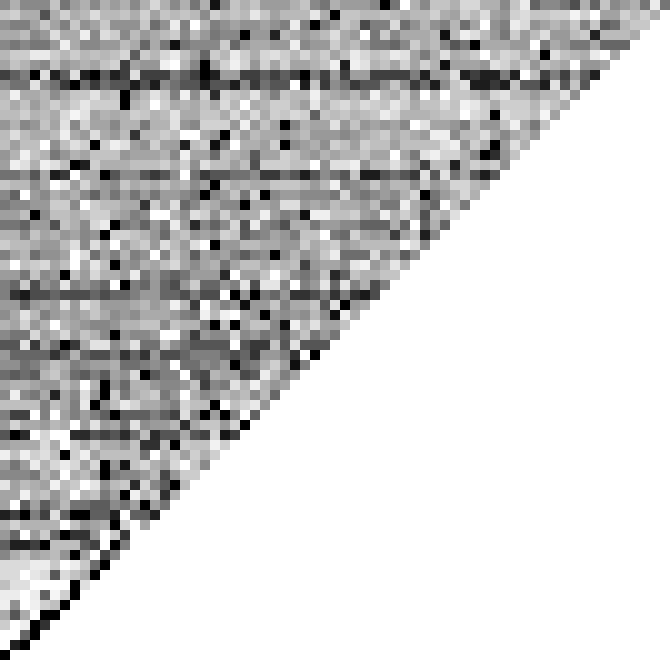
\includegraphics[width=0.4\linewidth]{images/cycling/high_config_20.png}
    %     \caption{Generation 20 for High Configuration}
    %     \label{fig:sfig3}
    % \end{subfigure}
    \begin{subfigure}{.4\textwidth}
        \centering
        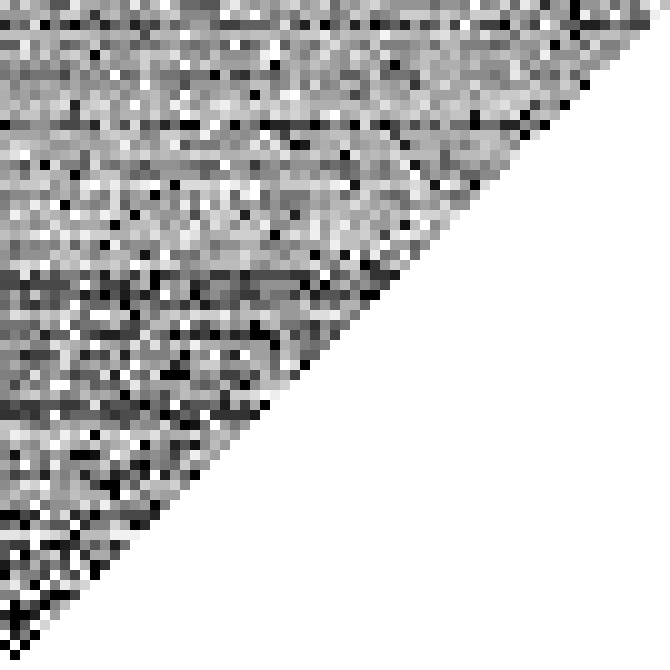
\includegraphics[width=0.4\linewidth]{images/cycling/high_config_7.png}
        \caption{Generation 7 for High Configuration}
        \label{fig:sfig4}
    \end{subfigure}
    \caption{Examples of Cycling}
    \label{ap_cyc}
\end{figure}

\begin{figure}[H]
    \begin{subfigure}{.4\textwidth}
        \centering
        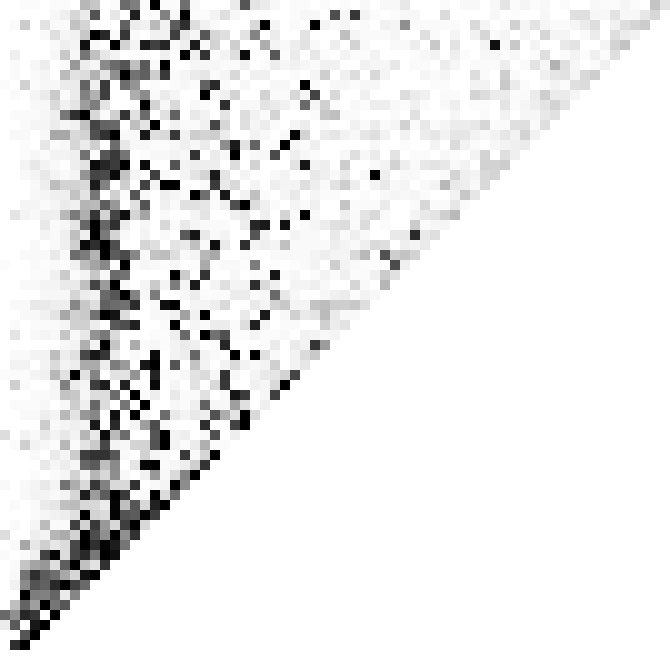
\includegraphics[width=0.4\linewidth]{images/disengagement/high_config13.png}
        \caption{Generation 13 for High Configuration}
        \label{fig:sfig1}
    \end{subfigure}
    \begin{subfigure}{.4\textwidth}
        \centering
        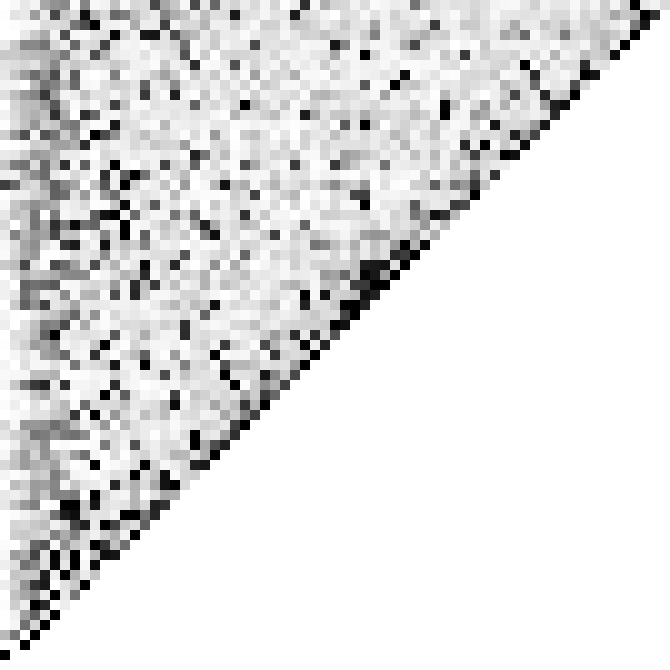
\includegraphics[width=0.4\linewidth]{images/disengagement/high_config22.png}
        \caption{Generation 22 for High Configuration}
        \label{fig:sfig2}
    \end{subfigure}
    \begin{subfigure}{.4\textwidth}
        \centering
        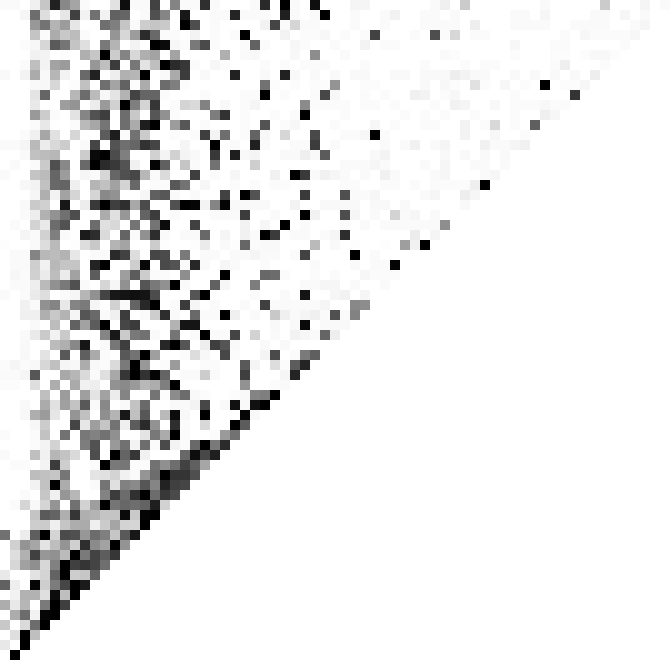
\includegraphics[width=0.4\linewidth]{images/disengagement/max_config3.png}
        \caption{Generation 3 for High Configuration}
        \label{fig:sfig4}
    \end{subfigure}
    \caption{Examples of Disengagement}
    \label{ap_dis}
\end{figure}

\begin{figure}[H]
    \begin{subfigure}{.4\textwidth}
        \centering
        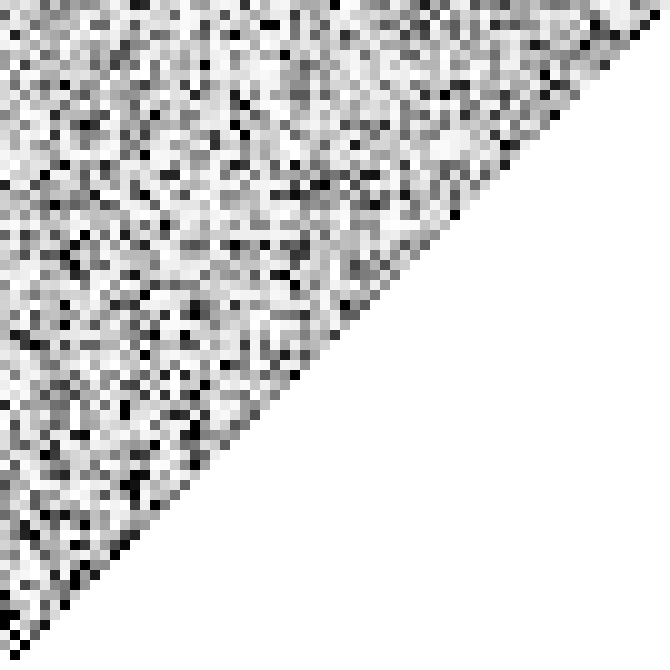
\includegraphics[width=0.4\linewidth]{images/mediocre/default_config_16.png}
        \caption{Generation 16 for High Configuration}
        \label{fig:sfig1}
    \end{subfigure}
    \begin{subfigure}{.4\textwidth}
        \centering
        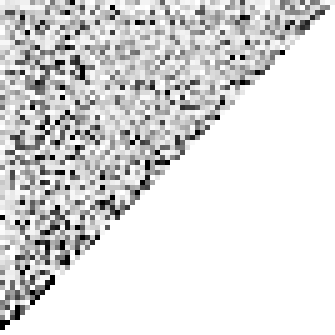
\includegraphics[width=0.4\linewidth]{images/mediocre/high_config_18.png}
        \caption{Generation 18 for High Configuration}
        \label{fig:sfig2}
    \end{subfigure}
    \begin{subfigure}{.4\textwidth}
        \centering
        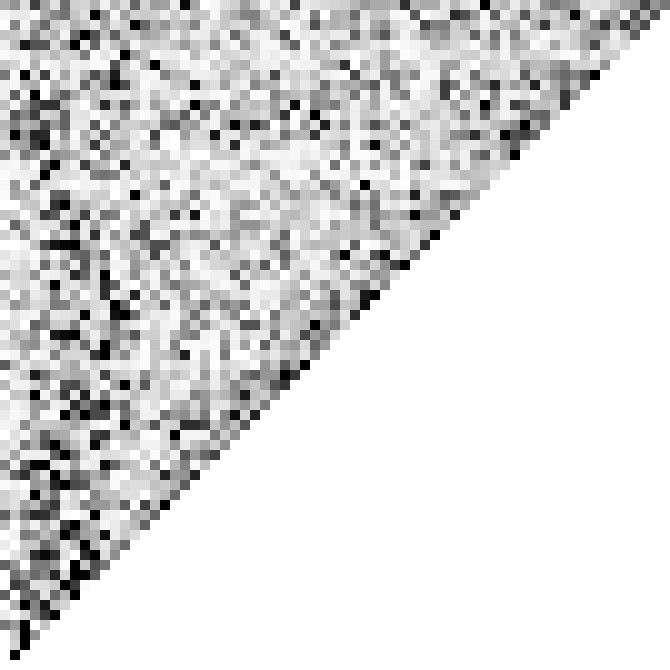
\includegraphics[width=0.4\linewidth]{images/mediocre/high_config_2.png}
        \caption{Generation 2 for High Configuration}
        \label{fig:sfig4}
    \end{subfigure}
    % \begin{subfigure}{.4\textwidth}
    %     \centering
    %     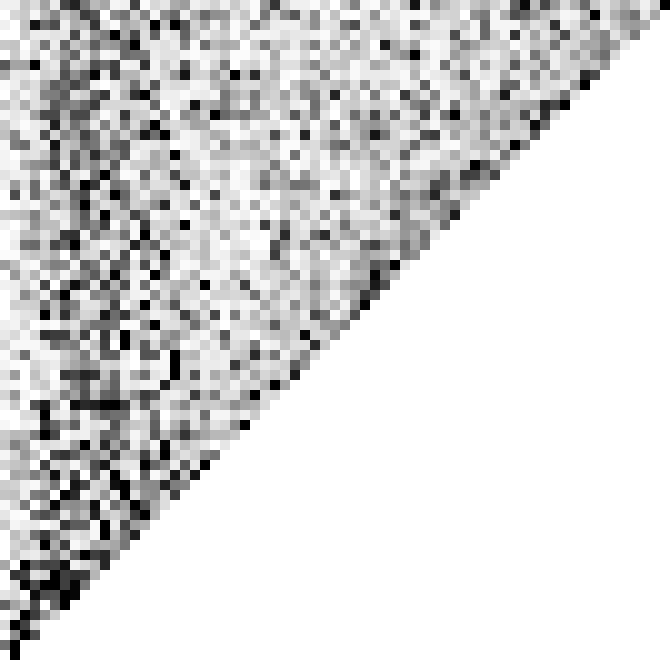
\includegraphics[width=0.4\linewidth]{images/mediocre/max_config_20.png}
    %     \caption{Generation 20 for Max Configuration}
    %     \label{fig:sfig4}
    % \end{subfigure}
    \caption{Examples of Mediocre Stability}
    \label{ap_med}
\end{figure}


\begin{figure}[H]
    \centering
    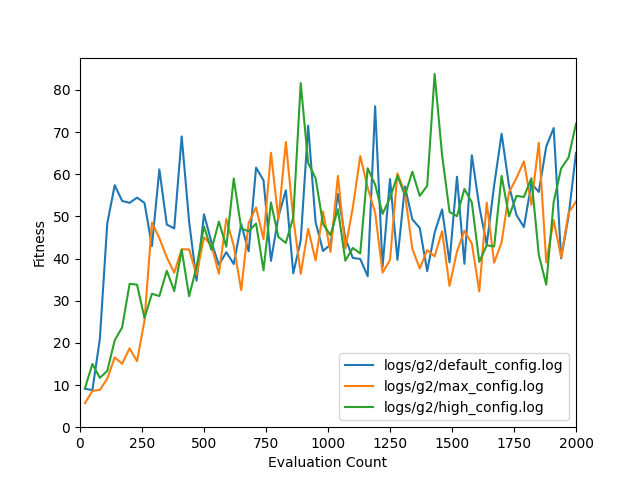
\includegraphics[width=1\linewidth]{images/graphs/config_compare_avg.png}
    \caption{Graph of all Configurations comparing their average fitness's}
    \label{config_avg}
\end{figure}

\begin{figure}[H]
    \centering
    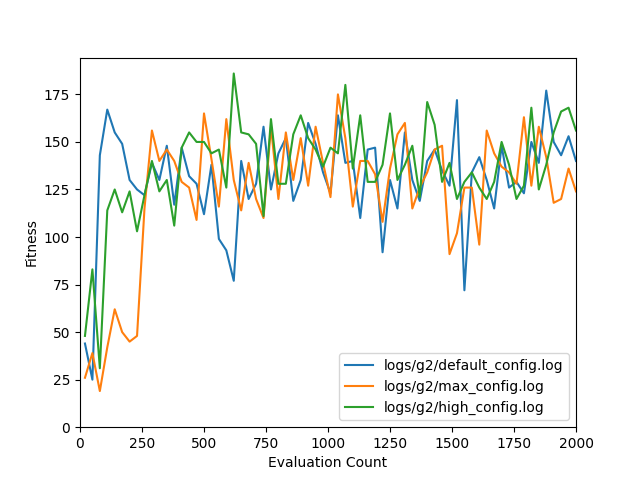
\includegraphics[width=1\linewidth]{images/graphs/config_compare_best.png}
    \caption{Graph of all Configurations comparing their best fitness's}
    \label{config_best}
\end{figure}


% \begin{lstlisting}[language=Python]
% def _turn(self, pacman_controller, ghost_controller):
%     """ Run a single turn through the pac-man game. """

%     # calculates best move for pac-man
%     move_scores = self._calculate_move_scores(pacman_controller, gpac.PACMAN)
%     pacman_move = self._select_best_move(move_scores, gpac.PACMAN)

%     # move ghosts
%     ghosts_moves = []
%     for ghost in gpac.GHOST:
%         move_scores = self._calculate_move_scores(ghost_controller, ghost)
%         ghost_move = self._select_best_move(move_scores, gpac.GHOST)
%         ghosts_moves.append(ghost_move)

%     # move pacman
%     self.game_instance.move(pacman_move, gpac.PACMAN)

%     # move ghosts
%     for move, ghost in zip(ghosts_moves, gpac.GHOST):
%         self.game_instance.move(move, ghost)

%     return self.game_instance.turn()
    
% def _generate_sensor_inputs(self, cell, unit):
%     """ Generates sensor inputs for a given location.

%     cell - location to calculate inputs on
%     """
%     if unit == gpac.PACMAN:
%         manhattan_ghost = self._closest_ghost(cell)
%         manhattan_pill = self._closest_pill(cell)
%         number_of_walls = self._calculate_adjacent_walls(cell)
%         manhattan_fruit = self._closest_fruit(cell)
%         ghost_shortest = self._shortest_ghost_distance(cell)
%         return [manhattan_ghost, manhattan_pill, number_of_walls, manhattan_fruit, ghost_shortest]
%     else:
%         manhattan_ghost = self._closest_ghost(cell)
%         manhattan_pacman = self._pacman_distance(cell)
%         shortest_pacman = self._shortest_pacman_distance(cell)
%         return [manhattan_ghost, manhattan_pacman, shortest_pacman]

% @ staticmethod
% def _select_best_move(move_scores, unit):
%     """ Selects best move out of selection of different scores each correlating to a move
%     direction.

%     move_scores - dictionary with keys of move direction and values of scores
%     relating to the move
%     """
%     compare = max if unit == gpac.PACMAN else min
%     max_score = compare(move_scores.values())
%     move = None
%     for move_direction in move_scores.keys():
%         if move_scores[move_direction] == max_score:
%             move = move_direction
%             break
%     return move

% def _calculate_move_scores(self, root_node, unit):
%     """ Calculates scores for every move Pac-Man can make based on weighted vector. """
%     move_choices = {}
%     for move in self.game_instance.get_spots_around_unit(unit):
%         sensor_values = self._generate_sensor_inputs(move, unit)

%         move_score = root_node.calculate(*sensor_values)

%         location = self.game_instance.locations[unit]
%         move_direction = self.game_instance.location_to_cardinal(location, move)

%         move_choices[move_direction] = move_score
%     return move_choices
% \end{lstlisting}